		\section{Nombre: Bolas de nieve}\label{obs.bolasN}
	\subsection{Descripción}
	Conjunto de nieve, su desplazamiento es vertical y tiene la capacidad de empujar al jugador hacia abajo tirándolo al vació. Su efecto no es constante, se activa y desactiva de manera periódica estando activo durante un tiempo determinado y desactivándose por otro tiempo determinado; los tiempos de actividad e inactividad pueden no ser los mismos. Para superar este obstáculo el jugador deberá aprovechar los tiempos de inactividad y cruzar la zona donde aparece la ráfaga.
	\subsection{Esquema}
Ver figura \ref{fig:bolasN}.
	\begin{figure}
  \centering
  \subfigure[El jugador se aproxima a la zona donde se ubica el obstáculo bolas de nieve.]{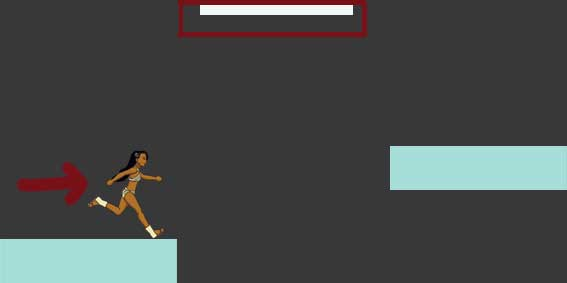
\includegraphics[width=0.3 \textwidth]{Imagenes/nieve01}}
   \subfigure [Se activan las bolas de nieve.]{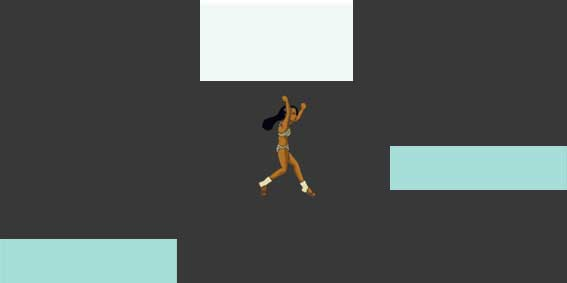
\includegraphics[width=0.3 \textwidth]{Imagenes/nieve02}}
    \subfigure [Las bolas de nieve empujan al jugador al vacío.]{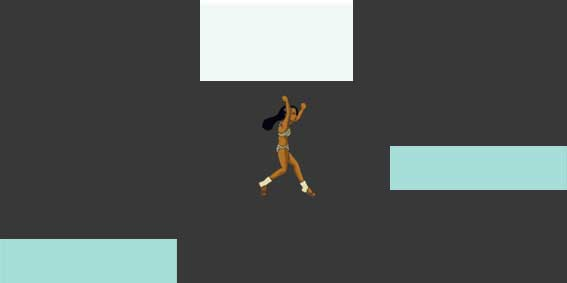
\includegraphics[width=0.3 \textwidth]{Imagenes/nieve02}}
  \caption{Bolas de nieve}
  \label{fig:bolasN}
\end{figure} 